\section{Аналитические раздел}

Команда разработчиков из 16 человек занимается созданием карты города на основе собственного модуля отображения. Проект должен быть завершен в течение 6 месяцев. Бюджет проекта: 50 000 рублей.

\section{Результаты работы}

Файл → Расписание
Указывается:
длительность работы в неделях, объем работ в часах, тип работ по умолчанию - с фиксированными трудозатратами (пункт 2);

1) количество рабочих часов в день - 8, количество рабочих часов в неделю - 40 (пункт 3);

2) начало рабочей недели в понедельник, а финансового года - в январе (пункт 4);

3) продолжительность рабочего дня с 9 до 18 часов (пункт 5).	

Проект → Изменить рабочее время

Указывается:

выходные и праздничные дни на ближайшие семь-восемь календарных месяцев от даты начала проекта (пункт 7).

\begin{figure}[ht!]
	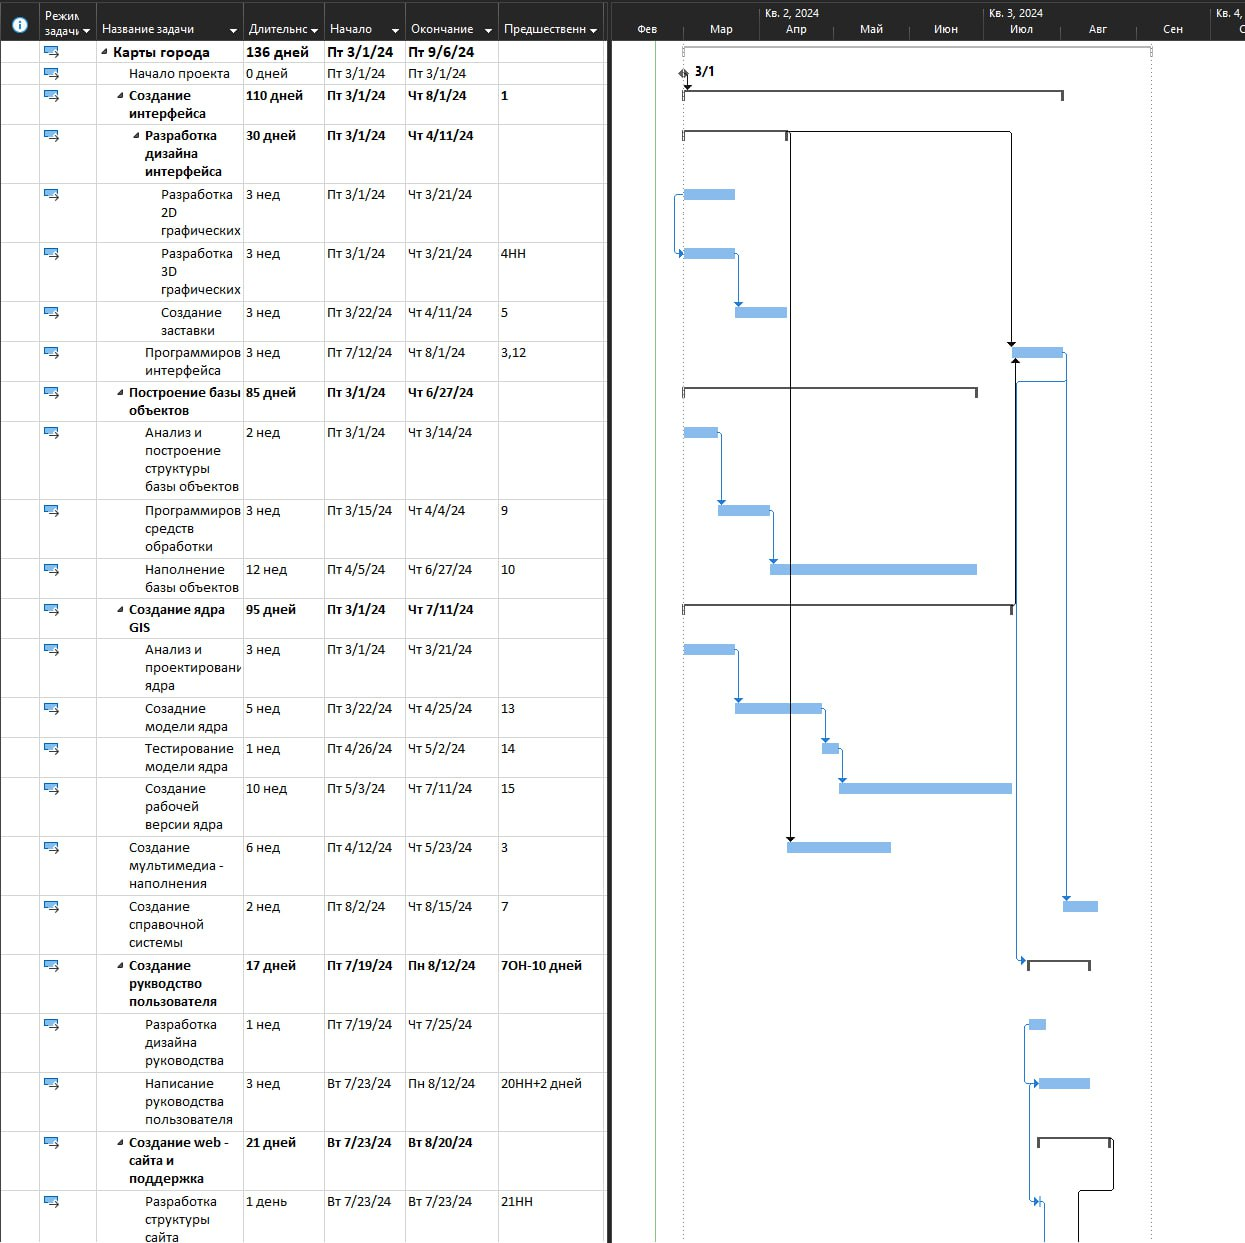
\includegraphics[width=0.75\linewidth]{assets/images/res1.jpg}
	\label{fig:r2}
	\caption{Первая часть диаграммы Ганта}
\end{figure}
\FloatBarrier
\begin{figure}[ht!]
	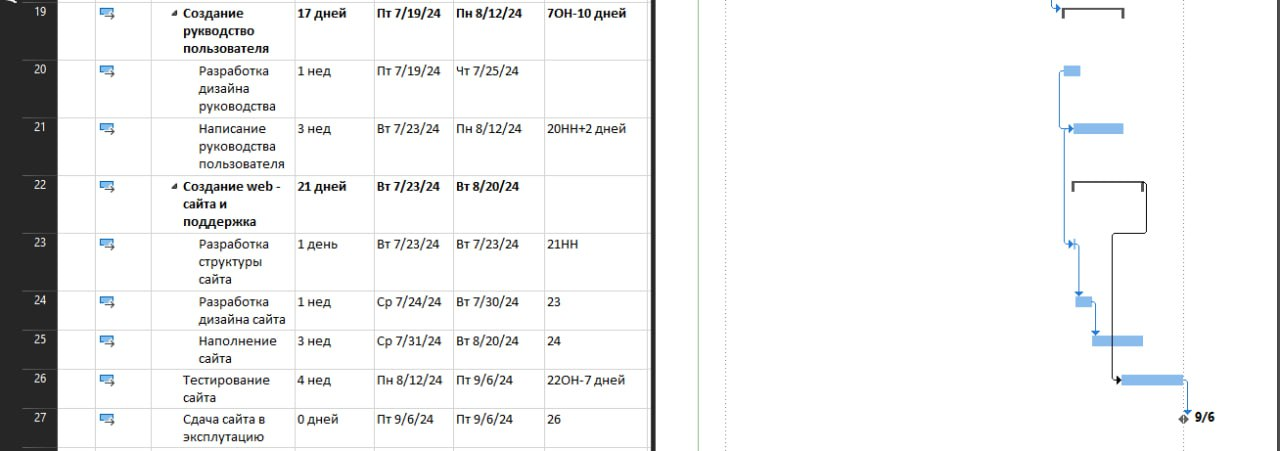
\includegraphics[width=0.75\linewidth]{assets/images/res2.jpg}
	\label{fig:r2}
	\caption{Вторая часть диаграммы Ганта}
\end{figure}
\FloatBarrier
Вывод:

Была проведена настройка рабочей среды, создание списка задач, его структурирование и установление связей между задачами.
В результате планирования выяснилось, что проект не будет закончен в заявленные сроки: заявленный срок – 03.09.2024, по расчетам получается 06.09.2024.